\chapter{場景建立}
\renewcommand{\baselinestretch}{10.0} %設定行距
\pagenumbering{arabic} %設定頁號阿拉伯數字
\setcounter{page}{1}  %設定頁數
\fontsize{14pt}{2.5pt}\sectionef
\section{前言}
老師有規定球場及球員的大小,重量\\
足球規格 (ball): 白色, 直徑 0.1m, 重量 0.5kg\\
足球場地 (field): 長 4m x 寬 2.5m\\
球門規格 (goal[0] and goal[1]: 長 0.6m, 高 0.3m, 寬 0.1m\\
球員尺寸範圍(player[0]-player[7]: 長寬高各 0.2m, 重量 5kg。\\
\section{建立球員}
我們使用CoppeliaSim來製作車子。\\
\

\begin{figure}[hbt!]
\begin{center}
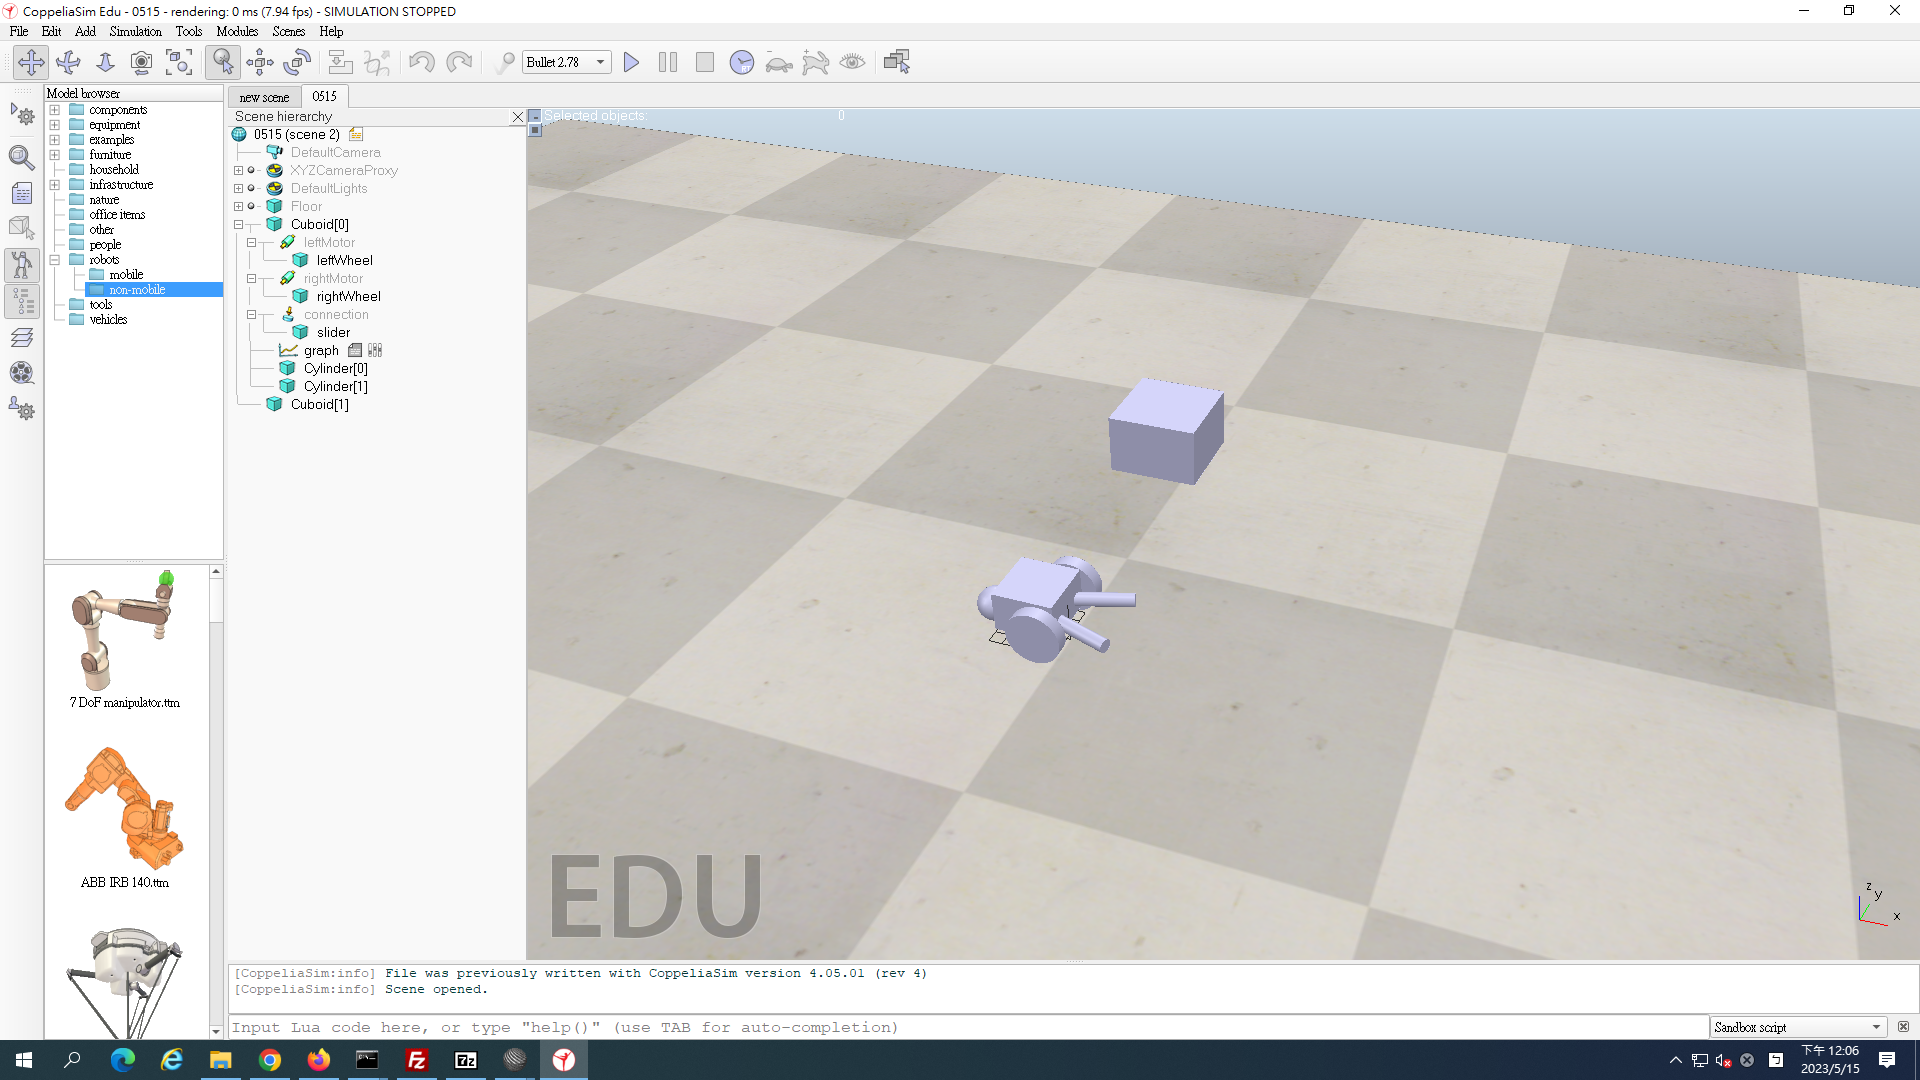
\includegraphics[width=10cm]{0515}
\caption{\Large 球員建立}\label{球員建立}
\end{center}
\end{figure}
\\
\
後發現在移動左右轉彎時會分解,因此直接在CoppeliaSim內修改了定位,且在後背加上號碼。如(圖.\ref{球員建立2})\\

\begin{figure}[hbt!]
\begin{center}
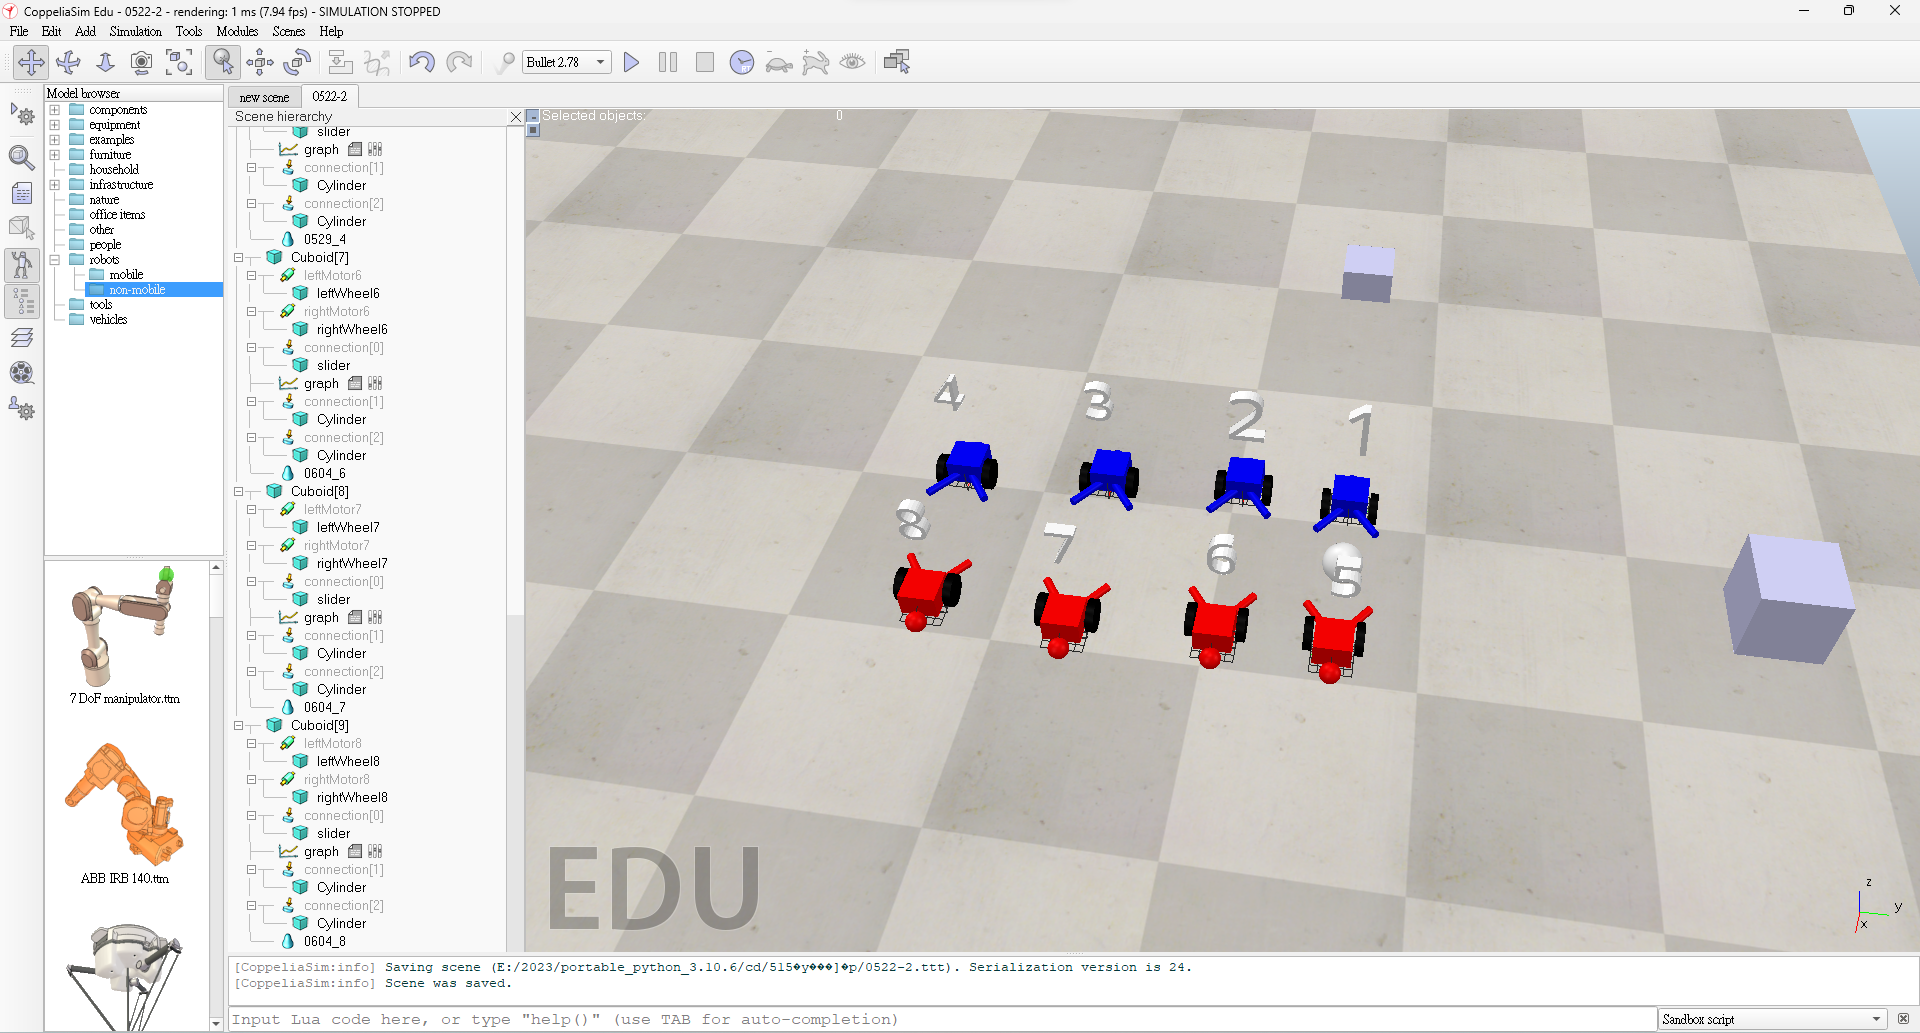
\includegraphics[width=10cm]{0604-1}
\caption{\Large 球員建立2}\label{球員建立2}
\end{center}
\end{figure}\

\section{建立記分板}
我們使用Onshape重新繪製了機械式記分板,如(圖.\ref{記分板建立})\\

\begin{figure}[hbt!]
\begin{center}
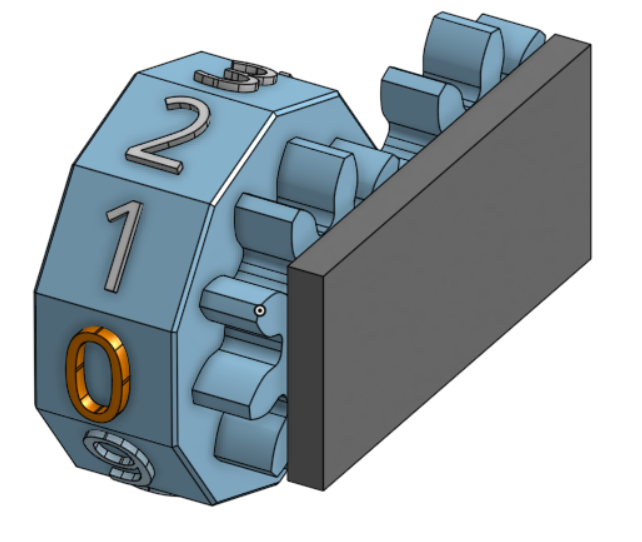
\includegraphics[width=10cm]{輪盤記分板-4-10teeth}
\caption{\Large 記分板建立}\label{記分板建立}
\end{center}
\end{figure}\

\begin{figure}[hbt!]
\begin{center}
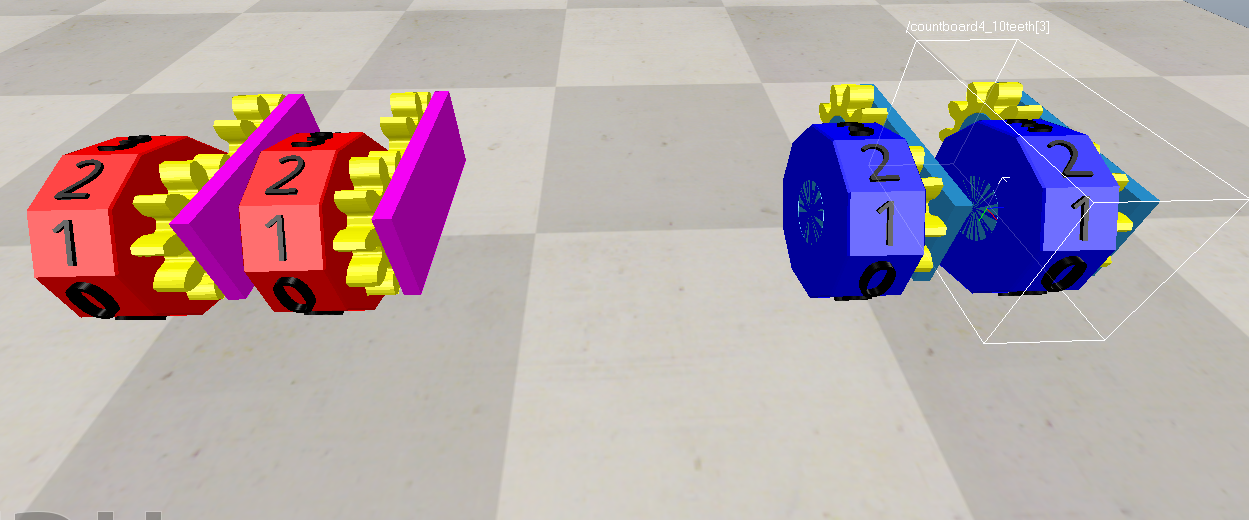
\includegraphics[width=10cm]{Screenshot 2023-05-29 113148.png4-10}
\caption{\Large 匯入記分板}\label{匯入記分板}
\end{center}
\end{figure}\
\newpage
\section{建立球場}
我們使用Onshape繪製了球場底板及球門,如(圖.\ref{球場繪製}),匯入CoppeliaSim後接著建立感測器,如(圖.\ref{建立球場})。\

\begin{figure}[hbt!]
\begin{center}
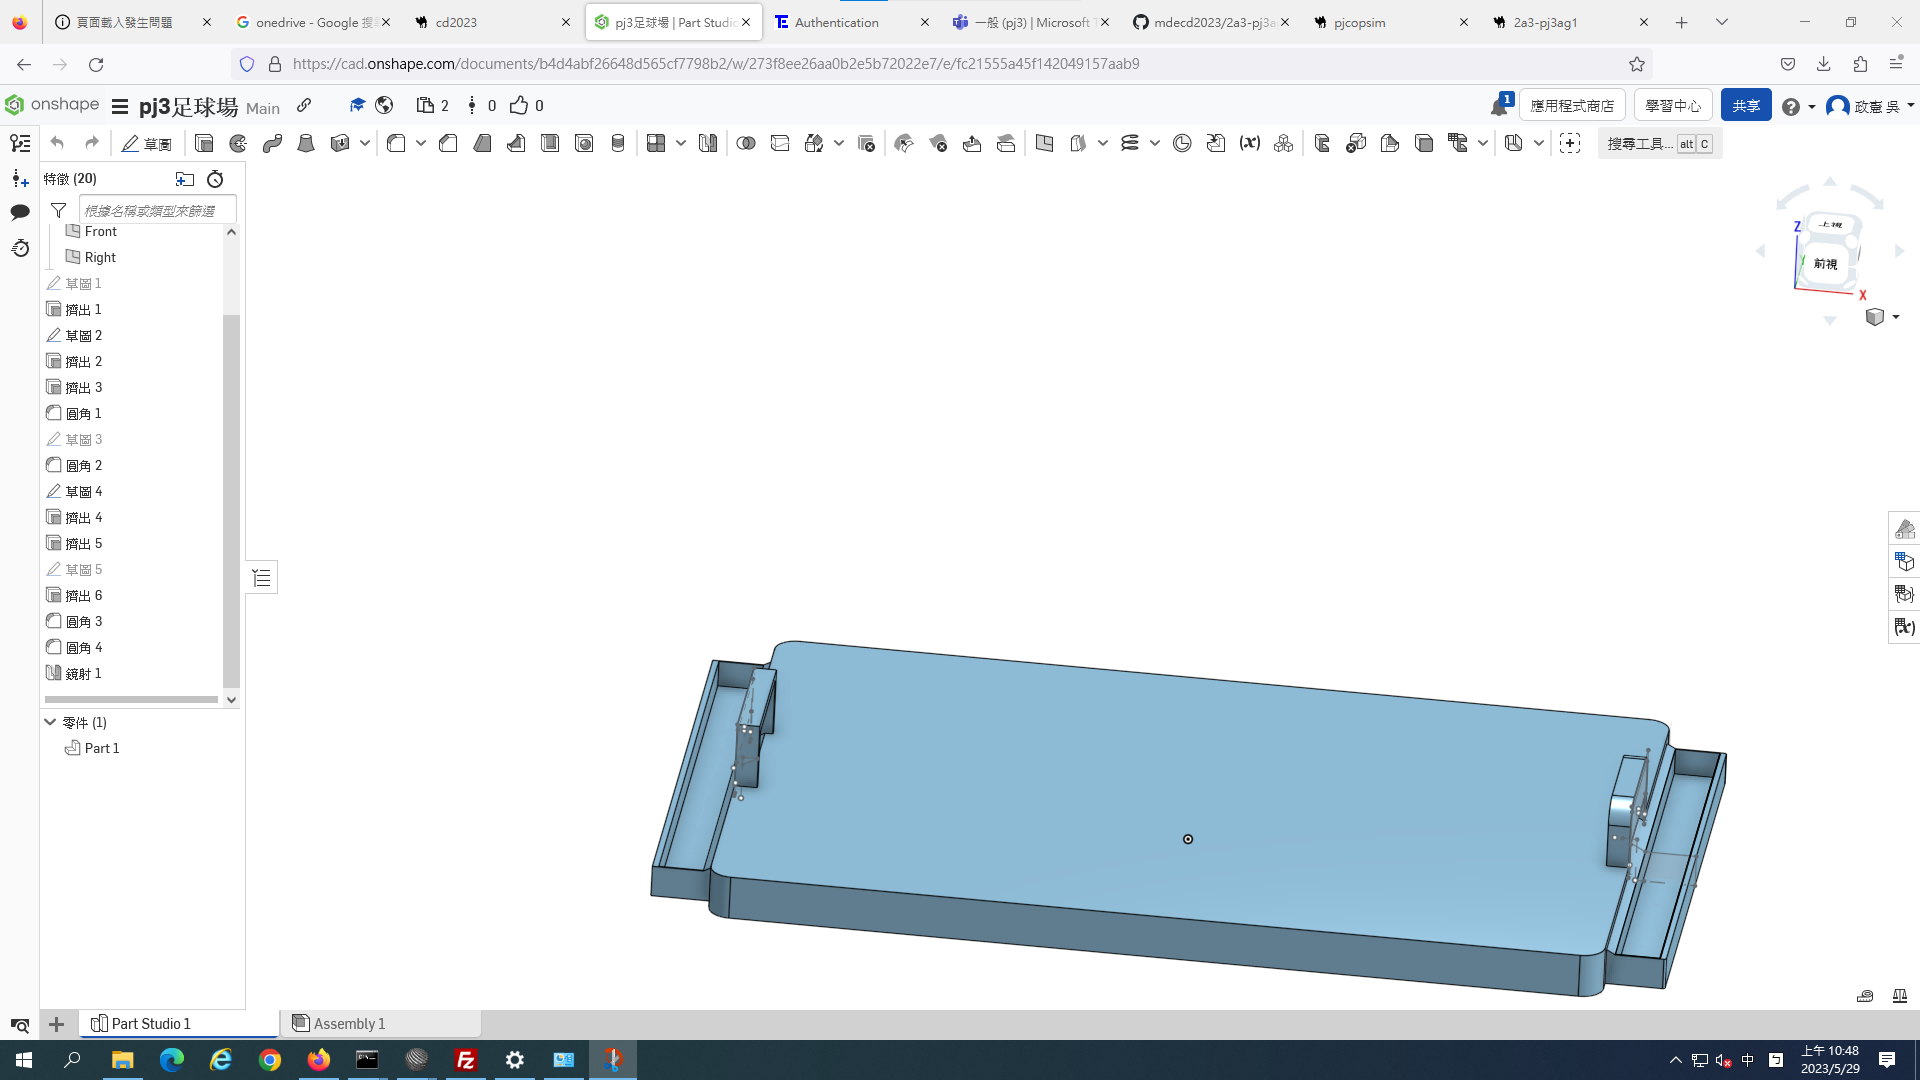
\includegraphics[width=8cm]{33333}
\caption{\Large 球場繪製}\label{球場繪製}
\end{center}
\end{figure}\


\begin{figure}[hbt!]
\begin{center}
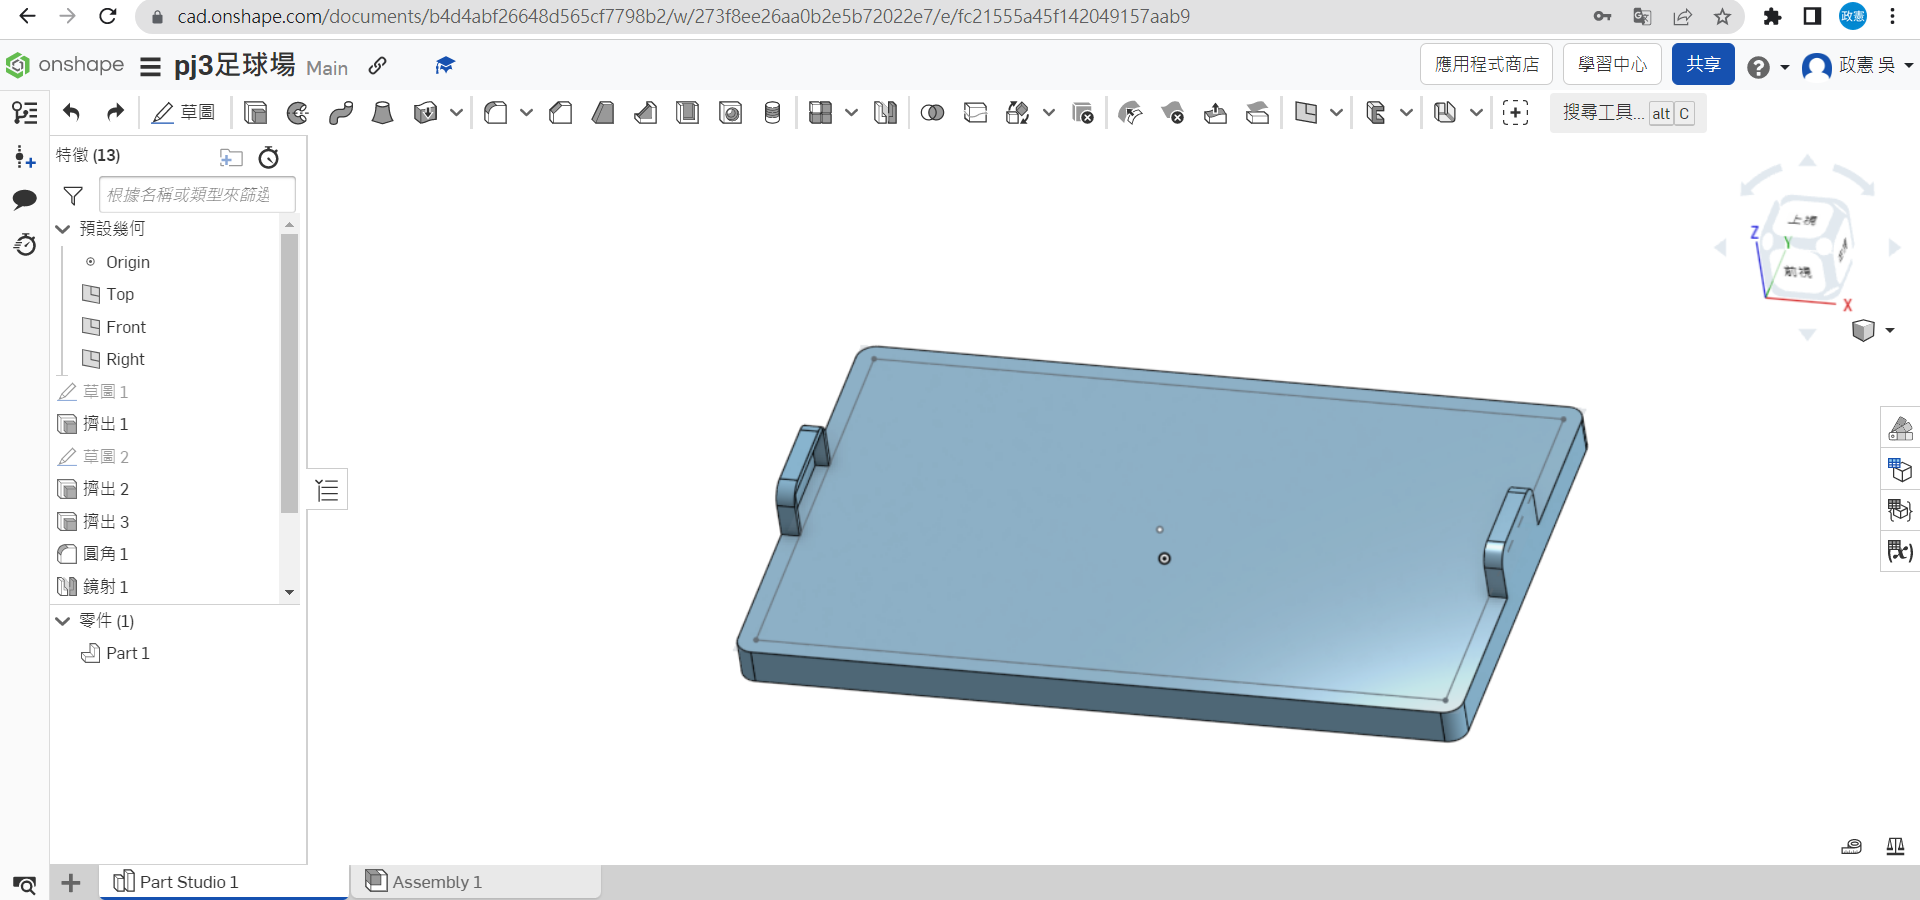
\includegraphics[width=8cm]{螢幕擷取畫面 2023-05-20 223657}
\caption{\Large 建立球場}\label{建立球場}
\end{center}
\end{figure}\

\newpage

